% REV00 Tue 20 Jul 2021 08:12:01 WIB
% START Tue 20 Jul 2021 08:12:01 WIB

\chapter{Sebelas}

% 11
\begin{figure}[htbp]
% h: here, where the figure appears in the text (use can always just use [h] )
% t: top,  top of the current page.
% b: bottom of the current page.
% p: page, top of the next available float space (sometimes end up being the end of the document).
\centerline{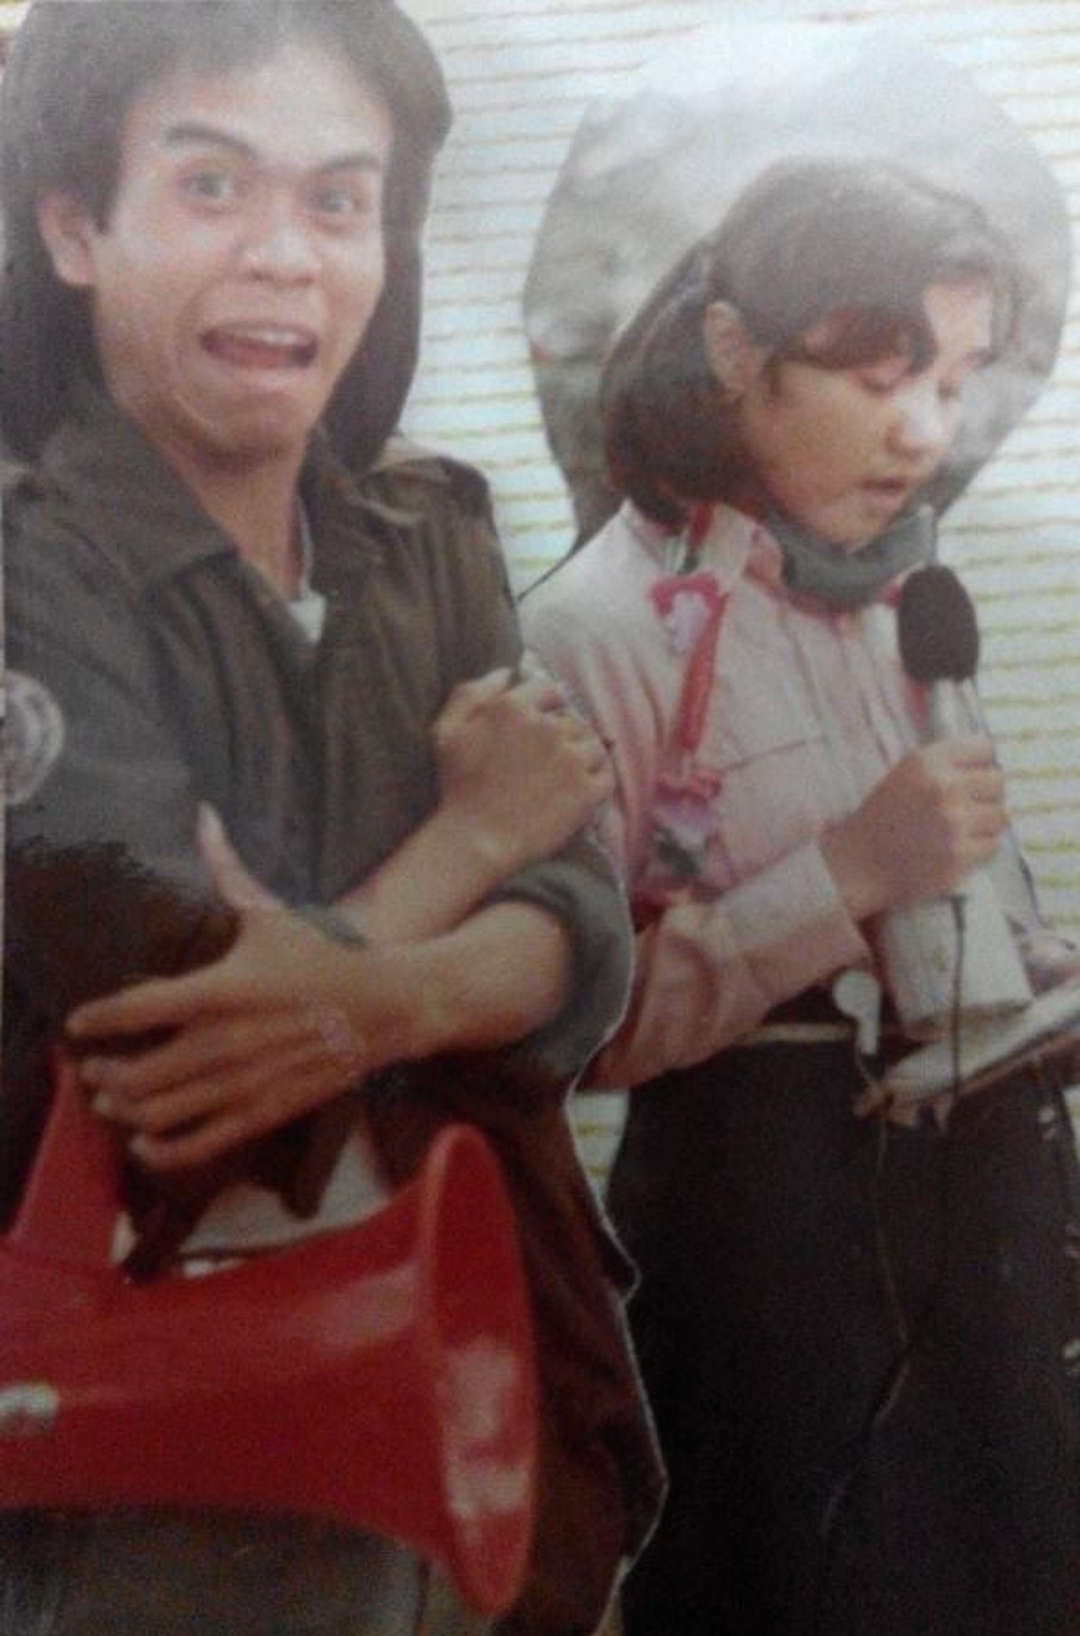
\includegraphics[scale=1.0]{01-11-01}}
\caption{"Satiri panitia OS 1982 seksi kesenian; dan Widya Lestari Fi’81 peserta OS" Sumber: Koleksi keluarga Kelvy Safira dan Fitria Clara Zora}
\label{01-11-01}
\end{figure}
%

Sejujurnya tidak ada yang begitu menarik di ITB bagi Satiri selain Fisika. Itupun perhatiannya harus ia bagi dengan anak-istrinya.

Padahal, di tahun 80an itu seingat saya terdaftar 83 unit kegiatan di ITB. Antara lain: Angklung, Bridge, Grup Apresiasi Sastra, Student English Forum, Phi Sigma Mu, Pramuka, dan Studi Teater Mahasiswa.

Semua jenis olah raga dan bela diri, dan bahkan Rugby juga ada. Seni daerah lumayan lengkap, ada Lingkung Seni Sunda, Maha Gotra Ganesha (Bali), Karawitan Jawa, dan UKM Minang. Di sini mahasiswa Sujiwo Tejo, yang kemudian memilih menjadi seniman dari pada jadi tukang insinyur, melahirkan Ludruk ITB pada tahun 1984.

Di sini juga ada PSIK menjadi think tank pergerakan mahasiswa di bawah KM dan DM ITB, yang belakangan hari dengan berat hati berubah menjadi KPM ITB.

Kegiatan-kegiatan itu bisa membuat anda tersesat, atau mungkin sebaliknya membuat anda menjadi manusia.

Maka, Satiri tidak ada di sana. Dia ada di Rawa Belong.

Jadi, selain kuliah apalagi yang menarik bagi Satiri? Cuma dua: Dangdut dan film India.

Kalau kita sedang di rumah Boy di Gardu Jati, itu kesempatan untuk nonton film India di bioskop “Taman Riang”. Anda yang orang Bandung tahu bioskop itu dimana? Ya, tepat di seberang Stasiun Hall (Cion, cion, cioon…). Ini bioskop yang kita boleh masuk dan keluar kapan saya.

Kalau jagoannya muncul semua penonton pukul-pukul bangku yang terbuat dari kaleng. Ribut. Banyak bangku yang rusak, banyak bangsat dan tumbila serta kecoa… Hahahah…

Saya pernah ikut nonton. Film India itu biasanya tiga jam, bertele-tele. Membuai saya untuk lelap tertidur, dan membuai Satiri untuk tetap konsen. Setelah nonton, kalau Boy lagi punya uang kita diajak makan di restorannya si Uni di St. Hall itu. Lamak banaa…

(Prof FPZ dan Uda S yang sekarang bekerja di IAEA, Austria, tidak mampu untuk melupakan warung Padang kecil itu)

Pernah juga kita ajak Satiri nonton film barat “Terms of Endearment” di bioskop Kings, alun-alun.

(Tahun 70, 80 dan 90an adalah tahun-tahun emas bisnis bioskop. Terutama di Bandung, yang rakyatnya gila nonton. Setelah periode itu semuanya digulung monopoli 21).

Film peraih 5 Oscar itu dibintangi oleh Debra Winger, Shirley MacLaine dan Jack Nicholson. Di akhir film, Satiri cuma bilang:

“Happy ending-nya sedih euy…” Huahahahah…

Hal-hal sepele begini, dan terutama seringnya kita lapar berjamaah, adalah hal-hal esensial yang menghubungkan umat manusia.

***

Pagi itu Satiri melewati "Dinding Ratapan Fisika" dari arah perpustakaan menuju Ruang TU dan R.1201 (Lab. Bosscha). Ya, betul, inilah dinding tempat meratap kedua setelah the Wailing Wall (Ha’it Al-Buraq atau the Kotel) yang ada di Kotatua Yerusalem itu.

Di sinilah tempat untuk menghempaskan kesombongan “Putera-puteri Terbaik Indonesia” (begitulah bunyi spanduk yang terpampang di avenue kampus Ganesha menyambut kita masuk ITB). Yang dulu juara SMA, juara se-kabupaten, atau bahkan juara se-propinsi, untuk pertama kali dalam hidupnya mendapati namanya ditempeli nilai 40 atau lebih rendah di dinding ini.

Melihat pengumuman nilai di Dinding Ratapan ini, tidak sedikit mahasiswa yang melengos, berjalan gontai menunduk, nanar, menatapi ubin kotak-kotak kecil warna kuning. Pening. Nyaris pingsan. Seraya menelan kesombongannya.

Hari itu belum lagi musim ujian. Hanya ada satu pengumuman yang selintas dilirik Satiri: Tulisan berwarna biru dengan huruf S di depannya.

Angin pagi yang segar membawa dua orang pakar dari Schumberger ke departemen Fisika: Pamer teknologi, pamer ilmu, plus mencari bibit unggul yang mau dijadikan kuli perusahaan. Acara itu nama kerennya open house: Yang ada di pengumuman itu.

Mau ikut kursus atau open house?

Take it or leave it? Sama persis polanya ketika dia harus memilih untuk menikahi Fitria pada saat itu juga, atau melupakannya selama-lamanya.

Maka Satiri memilih ikut rangkaian acara open house. Terpukaulah dia dengan presentasi bule-bule itu tentang bagaimana alat-alat canggih sistem wireline mereka untuk membuktikan banyak atau sedikitnya kandungan minyak di dalam perut bumi.

(MINYAK? Anda tentu ingat yang ditanyakan Satiri kecil kepada Bang Ipul, gurunya yang pertama).

% 11
\begin{figure}[htbp]
% h: here, where the figure appears in the text (use can always just use [h] )
% t: top,  top of the current page.
% b: bottom of the current page.
% p: page, top of the next available float space (sometimes end up being the end of the document).
\centerline{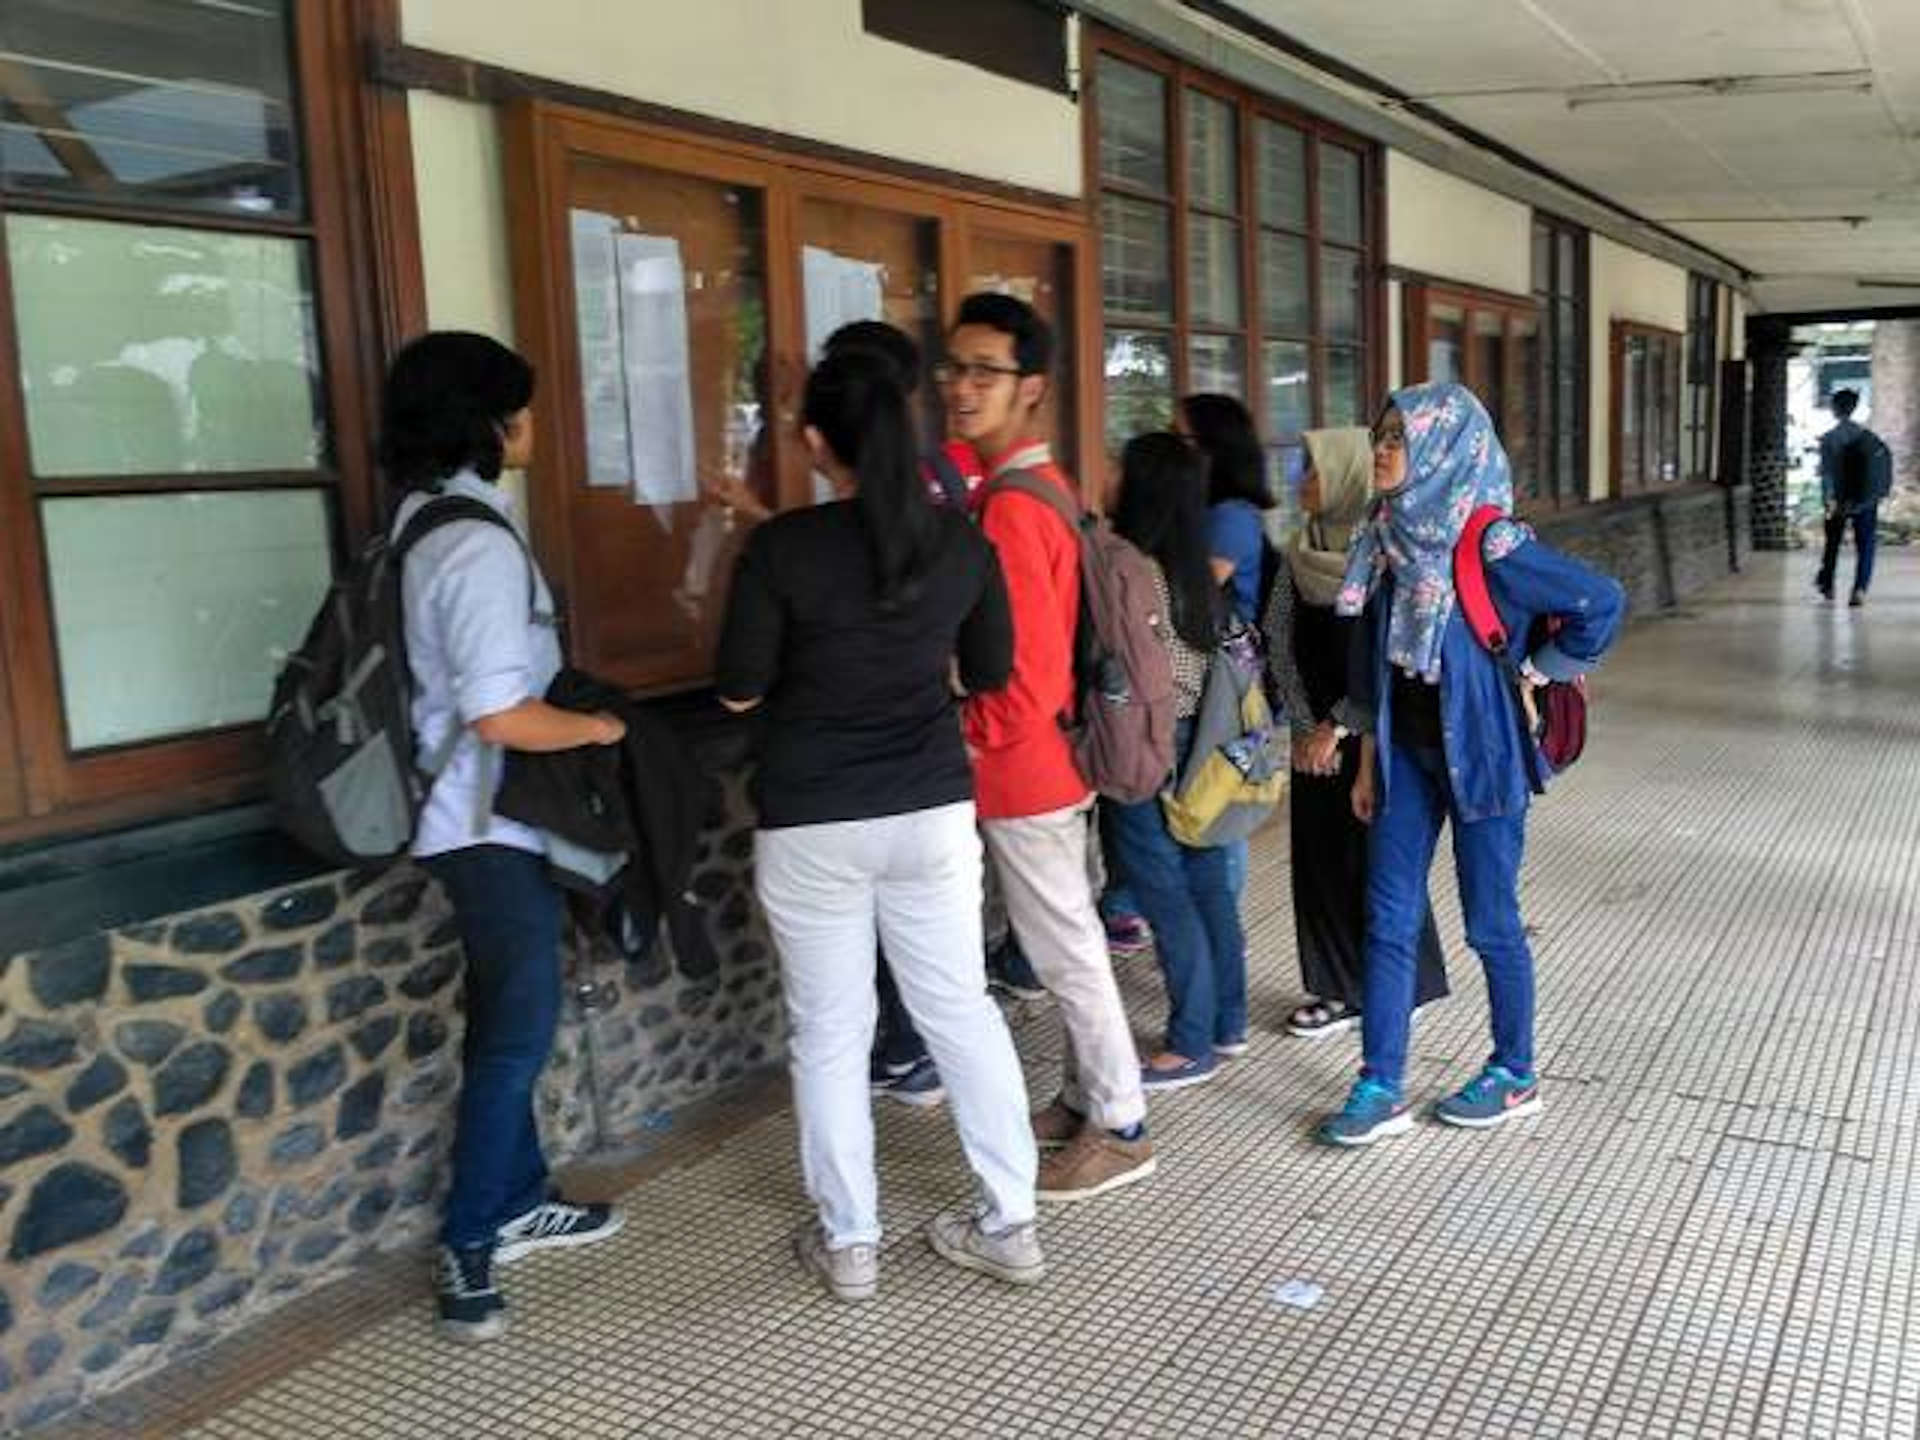
\includegraphics[scale=0.2]{01-11-02}}
\caption{"Dinding Ratapan Fisika" (Rinaldi Munir)}
\label{01-11-02}
\end{figure}
%

Ck, ck, ck, ck… Fantastic man! Siapa pula yang tidak kenal raksasa seperti Schlumberger wireline?

Antara sekilas dan sekejap Satiri masih sadar bahwa dia terikat kontrak untuk kursus bahasa Inggris, kuliah S2 dan S3 di Australia, dan menjadi dosen UB. Kontrak yang juga ditandatangani Kepada Departemen Fisika, Pak LH. Siapa tak kenal ilmuwan kaliber internasional bidang Fisika Bumi ini?

Usai presentasi, diadakan walk-in interview. Hebat nian muslihat mereka ini… Tanpa sepenuhnya sadar, karena sudah mendapat mantra, guna-guna dan pesona, kaki Satiri menarik-nariknya masuk ke ruang wawancara. Kalau alam sadarnya sedang bekerja, manusia normal, tentu saja saat ini dia sedang berada di ruang kursus bahasa.

Masuklah dia ke sana. Dan ditanya:

“Ada suatu kolam teratai. Hari pertama bunganya hanya ada satu. Hari kedua bunganya menjadi dua. Hari ketiga bunganya 4. Hari keempat bunganya 8, dst. Hari ke 100 kolam itu penuh bunga. Oke.

Sekarang, kalau hari pertama bunganya sudah ada dua, pada hari keberapa kolam itu penuh bunga?”

Yaaah, tiga detik Satiri terpukau.. Ini koq pertanyaannya begini? Serius, bukan Fisika atau elektronika?

Tapi dia toh tertap harus menjawab. Setelah berpikir 13 detik, dia menjawab:

“X”.

“Okay very good. Now, my second question: Ini ada baterai 1,5 volt. Bagian positifnya kita sambung dengan resistor 100 ohm. Kalau di ujung lain resistor itu kita pasang voltmeter dengan ujung negatif dari baterai, berapa angka yang akan ditunjukkan voltmeter?”

Nah, ini baru elektronika. Baiklah…

“Y”, kata satiri dengan mantap dalam sekejap.

“Excellent. Kamu boleh segera bekerja di Slb!”

Hah, hanya njawab dua pertanyaan saja? Gila ini perusahaan. Betul apa?

“Ya, betul,” kata si bule seolah mampu membaca pikiran Satiri.

“Kamu isi form ini, nanti tunggu surat panggilan dari kami. Selamat yah…” katanya sambil mengulurkan tangannya mengajak berjabat tangan.

Walaupun Satiri anak kampung, dia juga tahu bahwa berjabatan tangan itu kontrak yang disaksikan Tuhan. Dia jadi ragu, bagaimana dengan kursus bahasa dan kontraknya UB? Tapi tangannya maju duluan sebelum pikirannya menyelesaikan pertanyaannya itu.

Take it or leave it man!

Diapun berjabatan tangan. Sama girangnya saat pertama kali menjabat tangan mertua: Penuh kemenangan!

Keluar dari ruangan itu dia jijingkrakan, girang alang-kepalang. Diberi selamat teman-teman, di depan Dinding Ratapan.

Walaupun sudah telat, ia tetap berjalan menuju ke lab bahasa. Sambil berpikir-pikir santai:

Kalau kerja di Slb pasti langsung jadi orang kaya. Bosen kan selama ini jadi orang miskin?

Kalau jadi dosen, jadi “Oemar Bakri” kata Iwan Fals, pasti banyak amal, masuk surga. Tapi butuh waktu rada lama untuk jadi orang kaya.

Kalau masuk Slb, pasti menyalahi kontrak dan menyakiti UB dan terutama Ketua Departemen, Pak LH. Lah, siapa suruh mereka sakit hati?

Beres. Urusan sepele begini tidak perlu lah merepotkan Tuhan. Tuhan, koq diminta memecahkan urusan sepele?

Betul saja. Ketika Pak LH tahu Satiri diterima di Slb, muntab lah beliau. Kantor cabang Slb di Jakarta langsung ditelfon, memberitahu bahwa Satiri sudah ada kontrak dengan UB; dan,

“…dia itu sudah punya anak-istri!” ujarnya.

Pak LH tentu jangan disalahkan. Mempan?

Jadi bagaimana mimpi ke Australia yang sudah di depan mata?
\\[10pt]

Sumber tulisan asli \url{https://www.facebook.com/reno.alamsyah.94/posts/10226567777246745}

